\chapter{Geometry reconstruction by lookup table}\label{ch:lookupTable}

\vspace{-1.5 em}
\begin{addmargin}[-0.5cm]{0cm}
  \minitoc
\end{addmargin}
\hrule
\vspace{1.5 em}

\noindent
We begin our attempts at reconstructing geometries by taking a very simple approach, by using a lookup table. Simulating Coulomb explosions is computationally cheap, so we can simulate the explosion of many geometries and create a large map of geometries to asymptotic momentum vectors. Then reconstructing a geometry is simply a matter of looking up the geometry that produces the closest momentum vector arrangement. In this chapter we will describe an implementation of this approach and report on the geometries reconstructed using it. This will lead us to some new insights regarding the geometry reconstruction problem in general, motivating further investigation and possible enhancements to the method. Finally we will investigate its drawbacks, which further motivate the need for a more advanced approach and lay the foundations for the next chapter (see chapter \ref{ch:optimization}). Before fully abandoning this approach, we will also discuss its usefulness in future applications.

First however, we will take a brief look at lookup tables and motivate the need for it by investigating the failures of a previous attempt employing the Nelder-Mead simplex method.

\section{An aside on lookup tables}
The idea of using a lookup table to speed up calculations is as old as mathematics itself with examples dating back to some of the earliest mathematical texts produced by ancient Egyptian scribes during the Twelfth Dynasty of Egypt (circa 1990--1800 BC) \citep[p. 1, footnote 4]{Neugebauer45}. The Egyptian Mathematical Leather Roll contains perhaps the first such complete table and tabulates 26 sums of unit fractions equaling another unit fraction. \citet{Glanville27} reports on the leather roll,\footnotemark~ housed at the British Museum, and gives a photograph (figure \ref{fig:EMLR}) and schematic (figure \ref{fig:EMLRschematic}) of the table.

\footnotetext{The Egyptian Mathematical Leather Roll (and the more famous Rhine Mathematical Papyrus) was brought to the British Museum in 1864, however it took decades before archaelogists knew how to treat the leather to prevent its disintegration upon unrolling it.}

An even more impressive lookup table is found in the extensive Rhind Mathematical Papyrus, which (seemingly) methodologically expresses the fractions $2/n$ for odd $n \in \lbrace 3, 5, \dots, 101 \rbrace$ as the sum of 2--4 unit fractions! \citet{Gillings82} reports extensively on this table and the several dozen problems posed and solved on the papyrus, making extensive use of the table. The same table, verbatim, has found to be in use by scribes more than a millenium after its creation suggesting that it was of great utility. To this day, scholars argue about exactly how the scribes knew to construct the table and what methods they used \citep{Gillings74,Abdulaziz08}. \citet{Neugebauer45} reports on mathematical cuneiform texts used by the ancient Babylonians during similar time periods. Apparently, we are far from being the first to utilize a lookup table to speed up calculations.

Of course, 
The most familiar lookup table may be the multiplication times table that every elementary school student is familiar where sets of two integers are mapped to their product. Lookup tables have been employed since antiquity and one of the earliest surviving examples is a 98-column multiplication table from 493 A.D. attributed to the Roman, Victorius of Aquitaine \citep{Maher01}. Before the advent of the calculator and for much of scientific history, extensive logarithm tables were used to look up their values to several decimal places and to speed up computations. The earliest such tables date back to the ancient greeks although they have since been lost, and the earliest surviving one is a sine table by the ancient Indian mathematician \={A}ryabha\d{t}a circa 499 C.E. \citep{Hayashi97}.

\begin{figure}
  \centering
  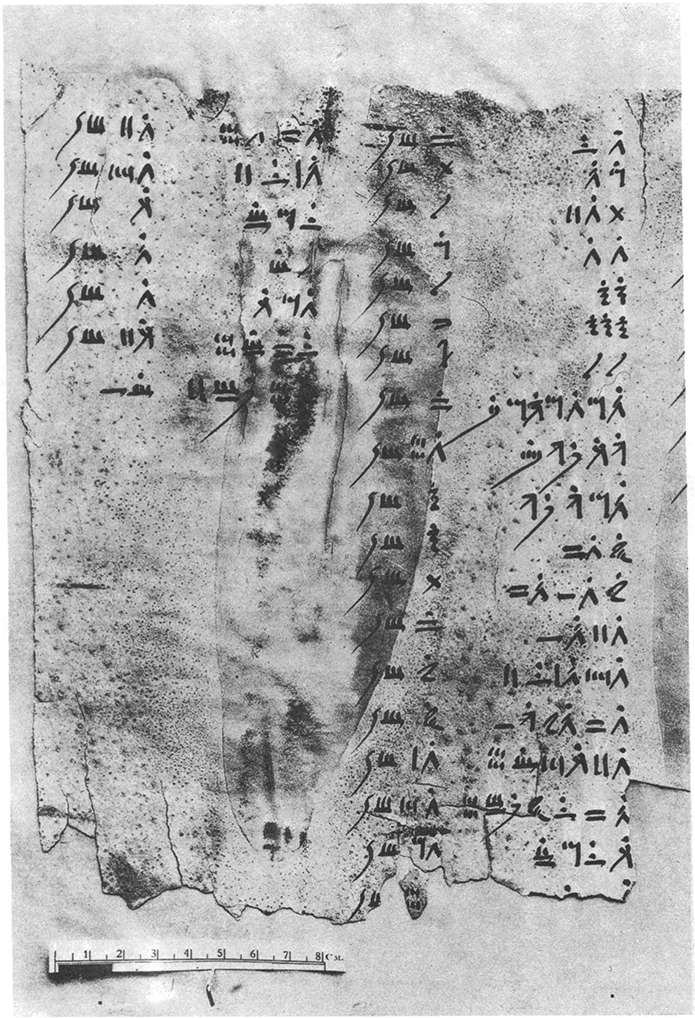
\includegraphics[width=\textwidth]{gfx/EMLR}
  \caption[Photograph of columns 3 and 4 of the Egyptian Mathematical Leather Roll.]
  {Photograph of columns 3 and 4 of the Egyptian Mathematical Leather Roll. Columns 3 and 4 are duplicates of columns 1 and 2. For example, row 9 of column 3 translates to $\displaystyle \frac{1}{50}\frac{1}{30}\frac{1}{150}\frac{1}{400} \quad \mathrm{it \; is} \quad \frac{1}{16}$ in modern notation where addition is implied. Figure \ref{fig:EMLRschematic} is a schematic of the table photographed here. Figure from \citet{Glanville27} which is accompanied by a translation.}
  \label{fig:EMLR}
\end{figure}

\begin{figure}
  \centering
  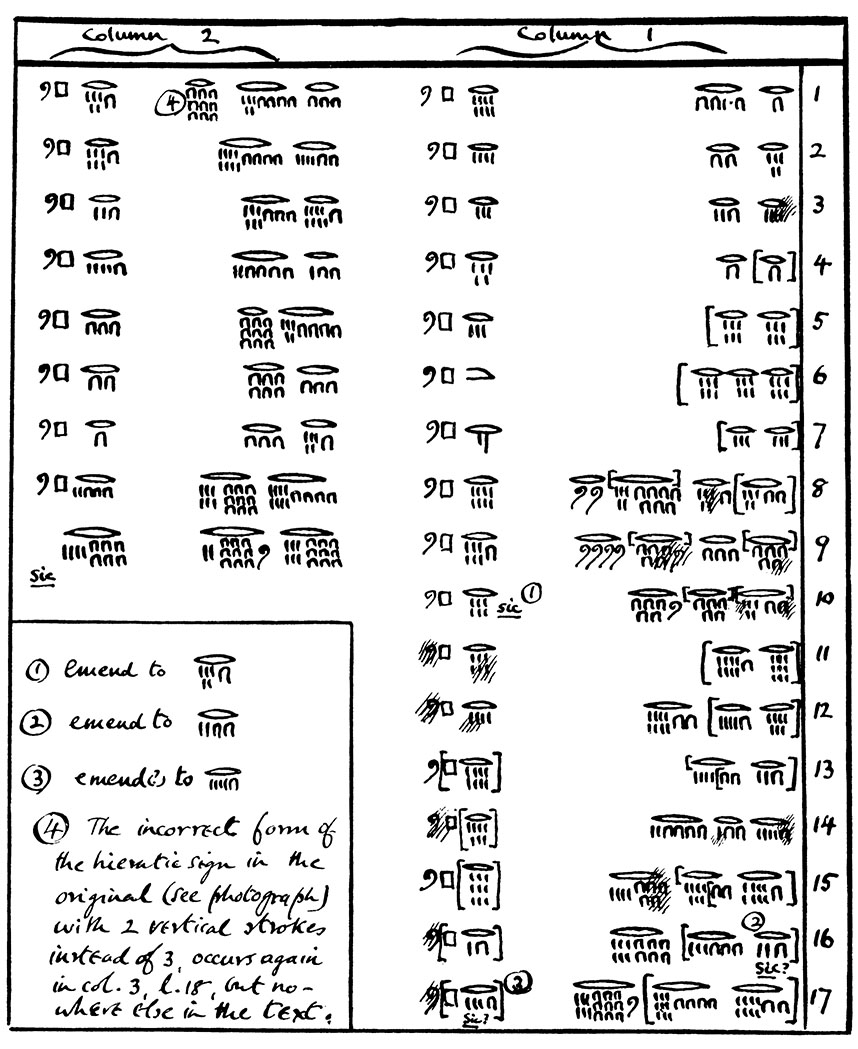
\includegraphics[width=\textwidth]{gfx/EMLRschematic}
  \caption[Schematic of columns 1 and 2 of the Egyptian Mathematical Leather Roll.]
  {Schematic of columns 1 and 2 of the Egyptian Mathematical Leather Roll. Columns 3 and 4 are duplicates of columns 1 and 2. Figure \ref{fig:EMLR} is a photograph of the table outlined here. Figure from \citet{Glanville27} which is accompanied by a translation.}
  \label{fig:EMLRschematic}
\end{figure}

Of course since then lookup tables have found an enormous number of uses in computer science. Arrays are ubiquitous objects in procedural programming languages and so is the more general dictionary object, especially in Python. Sine tables are still stored in calculators for quick trigonometric computations using the CORDIC algorithm and 3D lookup tables are used in image processing to store colormaps. In each case the speed offered by a lookup table once it has been generated is the main reason for their use.

\section{Previous attempt using the Nelder-Mead method}
\index{Simplex algorithm}
\index{Geometry reconstruction!Simplex algorithm}
\citet{Brichta09} proposed the reconstruction of small triatomic molecules using a simplex algorithm. It should not be confused with the more famous simplex algorithm, also an optimization algorithm but for linear programming, taught in almost every introductory optimization course. The algorithm employed should really should be referred to as the Nelder-Mead method, downhill simplex method, or amoeba method to avoid confusion between the two.\footnotemark

\footnotetext{We refer to it as the Nelder-Mead method for this chapter in alignment with Wikipedia.}

The Nelder-Mead algorithm is an ad-hoc or heuristic algorithm for nonlinear optimization that can be used without computing derivatives of the objective function\footnotemark. It was first generalized to minimizing functions by \citet{Nelder65} based off ideas by \citet{Spendley62}. It has enjoyed widespread popularity due to its ease of implementation and intuitive inner workings but it is not appropriate to every problem. In fact, it is not guaranteed to converge and thus fails when applied to some problems. It can even converge to non-stationary points in some cases \citep{McKinnon98}. Later publications would sometimes introduce tweaks to the Nelder-Mead method that would improve its performance on a specific problem. Unfortunately, I believe geometry reconstruction is not an appropriate problem for the Nelder-Mead method (see section \ref{ssec:simplexFail}).

\footnotetext{\citet{Wright10} provides a great discussion of the Nelder-Mead method, ending with a comment by John Nelder regarding his algorithm, ``Mathematicians hate it because you can’t prove convergence; engineers seem to love it because it often works.'' \citet[section 10.4]{NumericalRecipes} describes the algorithm in detail and provides a well-commented C++ implementation.}

\subsection{Previous reconstructions}
Unfortunately, \citet{Brichta09} only report on the reconstruction of molecular structures based on a few simulated geometries for carbon dioxide (\ch{CO2}) and formaldehyde (\ch{CH2O}). \citet{Brichta07} claims to have used this algorithm to report reconstructions of real \ch{CO2} geometries a couple of years earlier (see figure \ref{fig:simplexJPhysB}), which seems ripe for discussion and investigation, however the work is not even discussed. It was also used by \citet{Bocharova11} to report on the molecular structure of \ch{CO2} $(2,2,2)$ (see figure \ref{fig:simplexPRL}) however they do not report the set of geometries used to form the initial simplex. While they both produce a nice and intuitive plots, showing what appears to be an approximation to a molecular wavefunction with two broad position distributions, we will later see that this is deceptive and may not even represent physical geometries. 

\begin{figure}
  \centering
  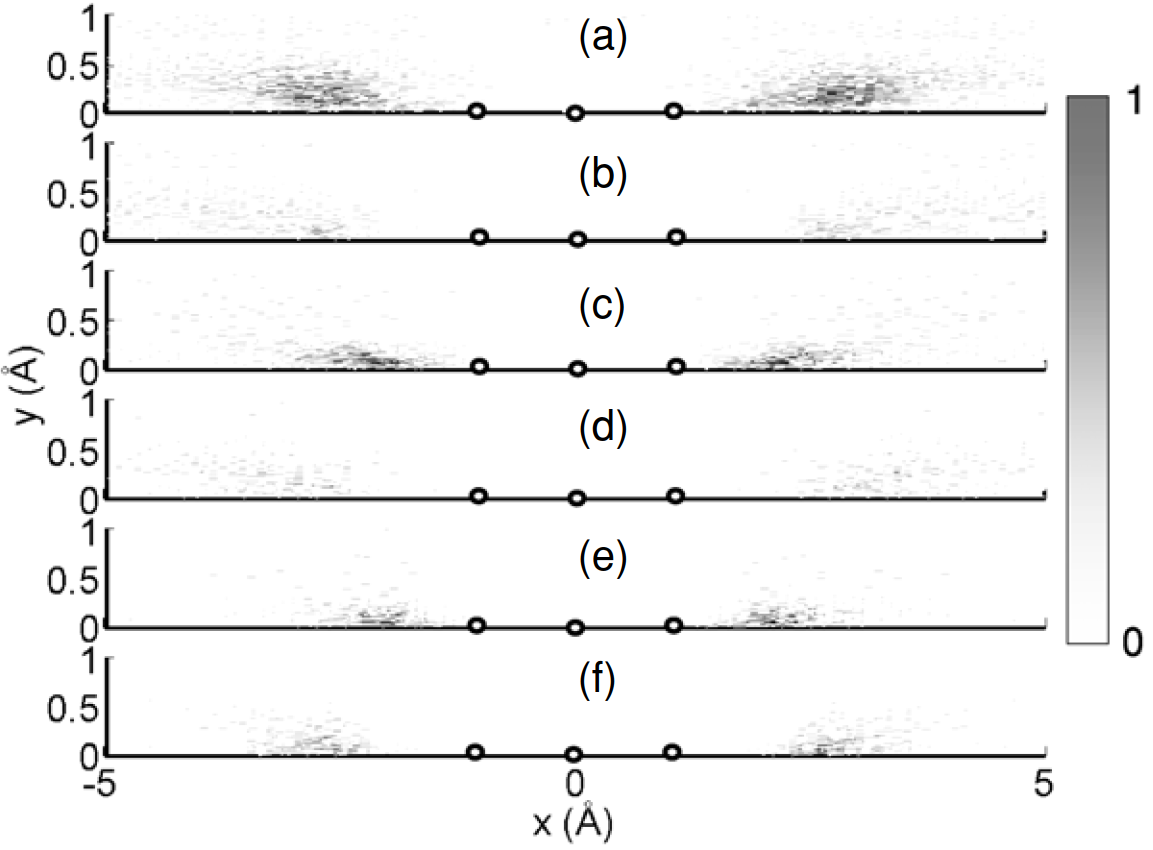
\includegraphics[width=\textwidth]{gfx/SimplexJPhysB}
  \caption[Reconstructed \ch{CO2} geometries using the Nelder-Mead method.]
  {Reconstructed \ch{CO2} geometries after Coulomb explosion by \SI{50}{\fs} laser pulses using the Nelder-Mead method for the (a) $(1,1,1)$, (b) $(1,2,1)$, (c) $(1,1,2)$, (d) $(1,2,2)$, (e) $(2,1,2)$, and (f) $(2,2,2)$ fragmentation channels. The carbon atom is placed at the origin with the higher charged oxygen atom in the +$x$-quadrant. The three circles represent the equilibrium or ground state geometry of \ch{CO2}, which is plotted as perfectly linear even though it should have a bond angle of \SI{172.5}{\degree} \citep{Siegmann02,Mathur92}. Each plot is reported to contain approximately $10^3$ events (or geometries), however it is hard to believe that (a) and (d) contain similar amounts of data. Figure from \citet{Brichta07}.}
  \label{fig:simplexJPhysB}
\end{figure}

\begin{SCfigure}
  \centering
  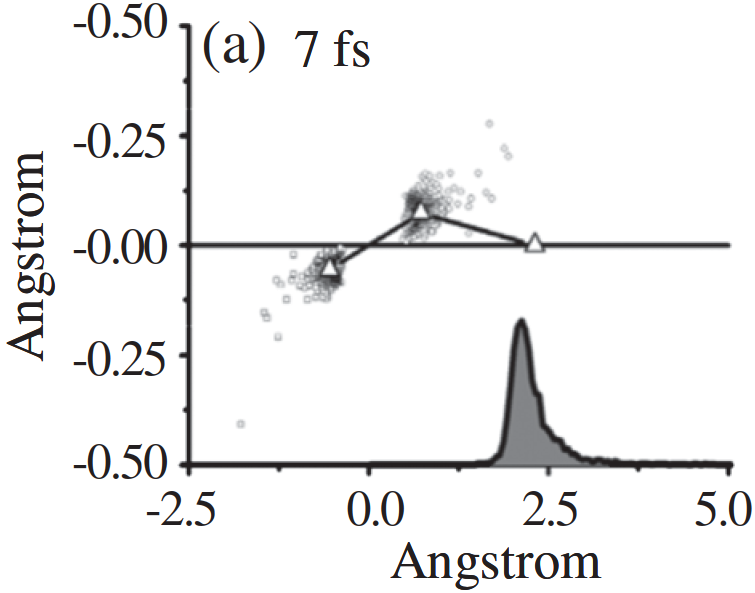
\includegraphics[width=0.5\textwidth]{gfx/SimplexPRL}
  \caption[Reconstructed \ch{CO2} in the $(2,2,2)$ charge state using the Nelder-Mead method.]
  {Reconstructed \ch{CO2} geometries in the $(2,2,2)$ charge state after explosion by a \SI{7}{\fs} laser pulse using the Nelder-Mead method. Although unreported, the triangles presumably pinpoint the centroid (or average) position of each atom while the the 
    
    They report a molecular geometry of $\langle r_\mathrm{CO} \rangle \approx \SI{1.3}{\angstrom}$, $\langle \theta_\mathrm{OCO} \rangle \approx 168\degree$ which is close the equilibrium geometry of $\langle r_\mathrm{CO} \rangle \approx \SI{1.16}{\angstrom}$ \citep{ChemistryOfTheElements} and $\langle \theta_\mathrm{OCO} \rangle \approx 172\degree$ \citep{Siegmann02,Mathur92}. Figure from \citet{Bocharova11}.}
  \label{fig:simplexPRL}
\end{SCfigure}

\subsection{Inability to reliably reconstruct asymmetric triatomic geometries} \label{ssec:simplexFail}

Simulated geometries are used for this analysis mainly because we can check exactly how far off the algorithm is from the correct solution. The simulated geometry only experiences the Coulomb force and so a solution is guaranteed by our classical simulation as no quantum mechanical effects occur. Simulated geometries are thus the easiest geometries to reconstruct and serious doubts regarding an algorithm's utility must be raised if it cannot reconstruct them. We do not know the geometries \textit{a priori} when reconstructing real geometries and so we need a trustworthy reconstruction algorithm in order to trust any geometries it produces.

\begin{figure}
  \centering
  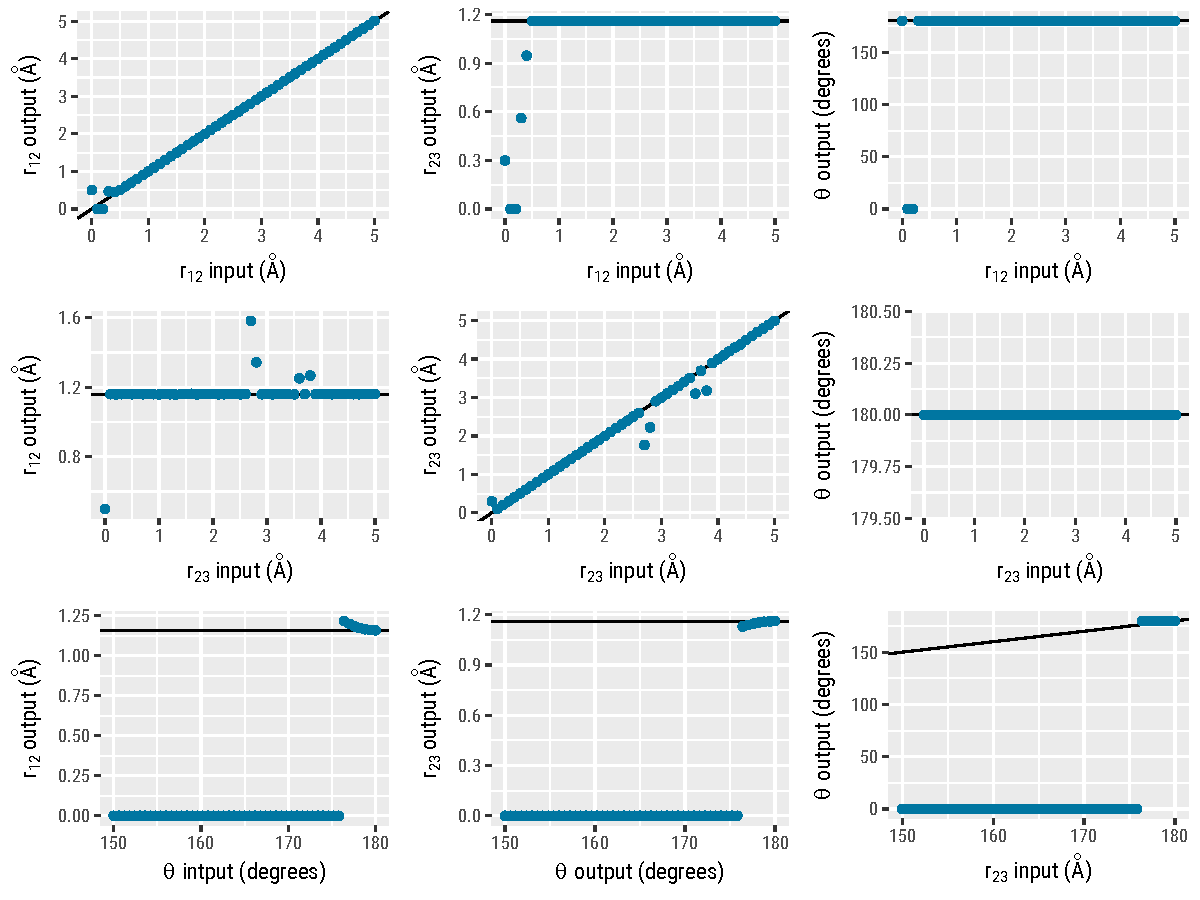
\includegraphics[width=\textwidth]{Plots/CO2SimplexCalibrationPlots}
  \caption[Testing the Nelder-Mead method's ability to reconstruct \ch{CO2} (2,2,2) geometries]
  {Testing the Nelder-Mead method's ability to reconstruct \ch{CO2} (2,2,2) geometries by starting with the ground-state geometry of \ch{CO2} and varying each parameter one-by-one. In the first row, the first \ch{C-O} bond length ($r_{12}$) was varied to create an ``input geometry'' which underwent a simulated Coulomb explosion. The resulting momentum vectors from the explosion were fed into the Nelder-Mead algorithm which converged to a geomety, the ``output geometry''. The second \ch{C-O} bond length ($r_{23}$) and the bond angle $\theta$ were varied in the second and third rows respectively. Solid black lines indicate the expected output geometry, so deviations indicate a failure on the algorithm's ability to reconstruct the geometry. We see that the algorithm can accurately reconstruct the geometry when a single bond length is varied but completely fails once the bond angle is below approximately $176\degree$, thus simply producing zeros.}
  \label{fig:CO2SimplexCalibrationPlots}
\end{figure}

\begin{figure}
  \centering
  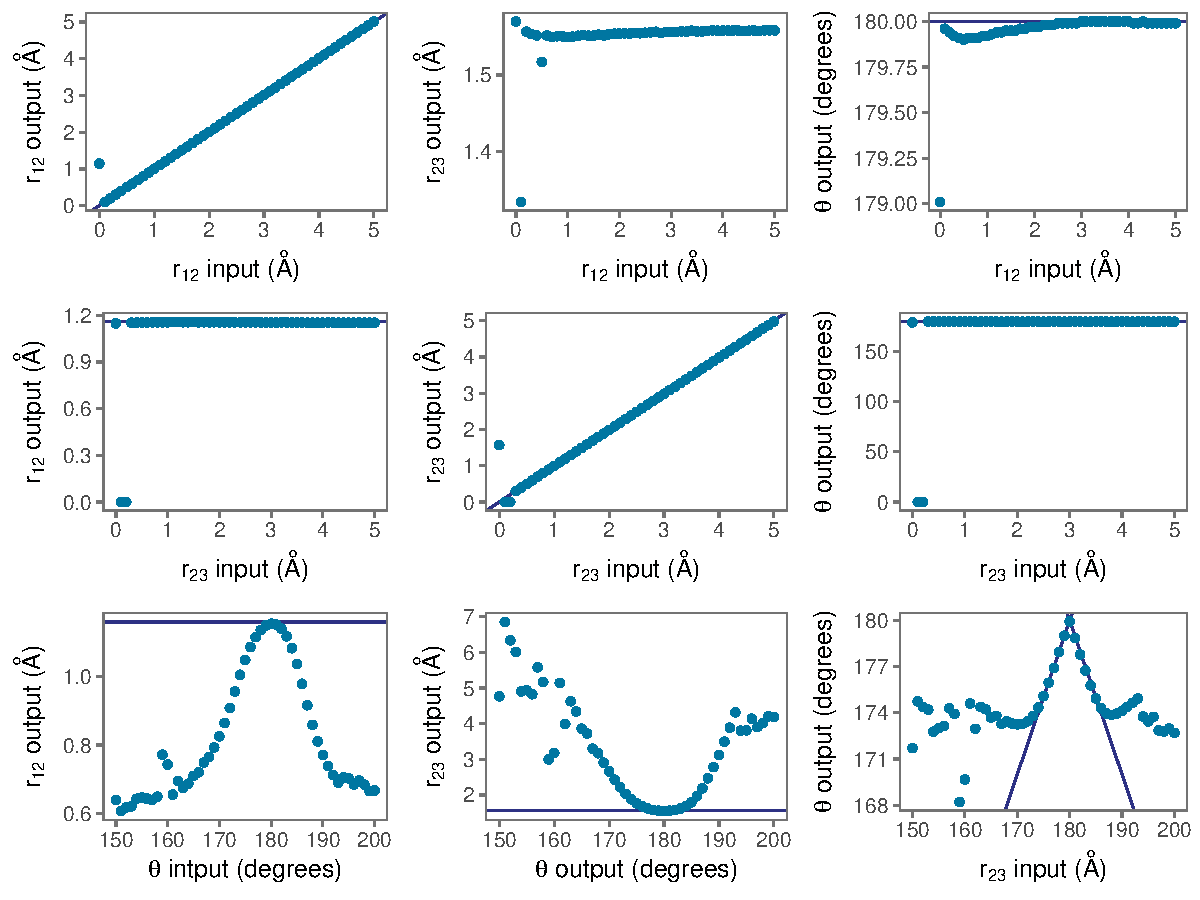
\includegraphics[width=\textwidth]{Plots/OCSSimplexCalibrationPlots}
  \caption[Testing the Nelder-Mead method's ability to reconstruct \ch{OCS} (2,2,2) geometries.]
  {Testing the Nelder-Mead method's ability to reconstruct \ch{OCS} (2,2,2) geometries by starting with the ground-state geometry of \ch{CO2} and varying each parameter one-by-one. In the first row, the \ch{C-O} bond length ($r{\textnormal{CO}}\equiv r_{12}$) was varied to create an ``input geometry'' which underwent a simulated Coulomb explosion. The resulting momentum vectors from the explosion were fed into the Nelder-Mead algorithm which converged to a geomety, the ``output geometry''. The \ch{C-S} bond length ($r{\textnormal{CS}}\equiv r_{23}$) and the bond angle $\theta$ were varied in the second and third rows respectively. Solid black lines indicate the expected output geometry, so deviations indicate a failure on the algorithm's ability to reconstruct the geometry. We see that the algorithm can accurately reconstruct the geometry when a single bond length is varied but performs worse and worse as the molecular bends, even slightly.}
  \label{fig:OCSSimplexCalibrationPlots}
\end{figure}

A more thorough analysis should vary multiple parameters at once, however if the algorithm cannot reconstruct geometries that different from the ground-state by a single parameter.

It should be noted that the Nelder-Mead algorithm, especially in our case, is quite sensitive to the geometries chosen to represent the initial simplex. Changing them could significantly impact the algorithm's ability to converge on the correct geometry. Of course, this does suggest that there may exist a set of initial geometries that significantly improve the algorithm's reliability, however, after many attempts I could not find such a set. Perhaps \citet{Brichta07} and \citet{Bocharova11} happened to find an optimal set of geometries, however no mention of it is made, casting doubts over their geometry reconstructions and any consequent conclusions. The neccessity of fine-tuning the Nelder-Mead method should immediately prompt the search for an improved method.

% Simplex: Very sensitive to initial conditions. Probably cannot reproduce same results. If we change it to optimize theta lines, the others get out of whack.

\pagebreak
\section{Exploratory data analysis of our measurements}

\begin{figure}
  \centering
  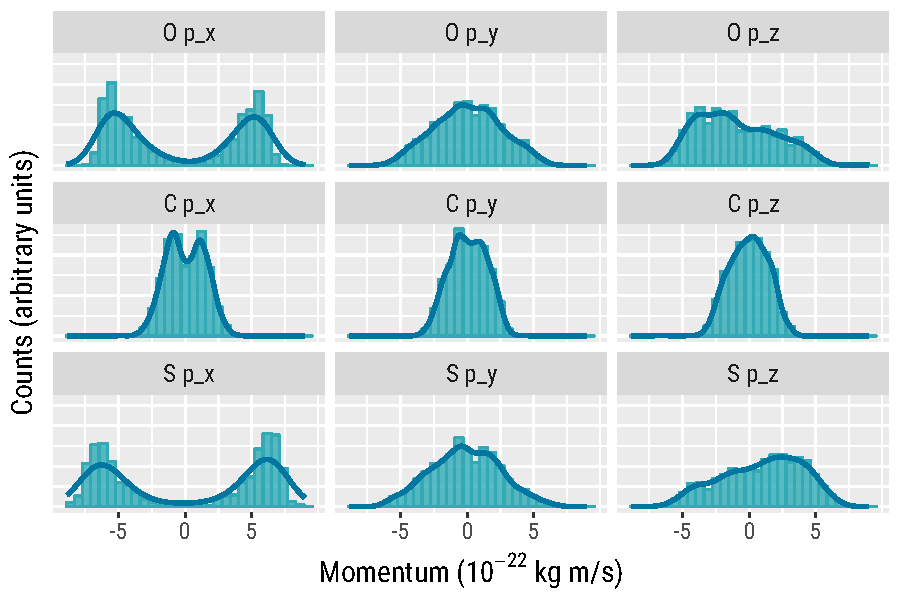
\includegraphics[width=\textwidth]{Plots/OCS2227fsMomentum}
  \caption[OCS (2,2,2) 7fs momentum.]
  {OCS (2,2,2) 7fs momentum.}
  \label{fig:OCS2227fsMomentum}
\end{figure}
\clearpage

\pagebreak
\begin{figure}
  \centering
  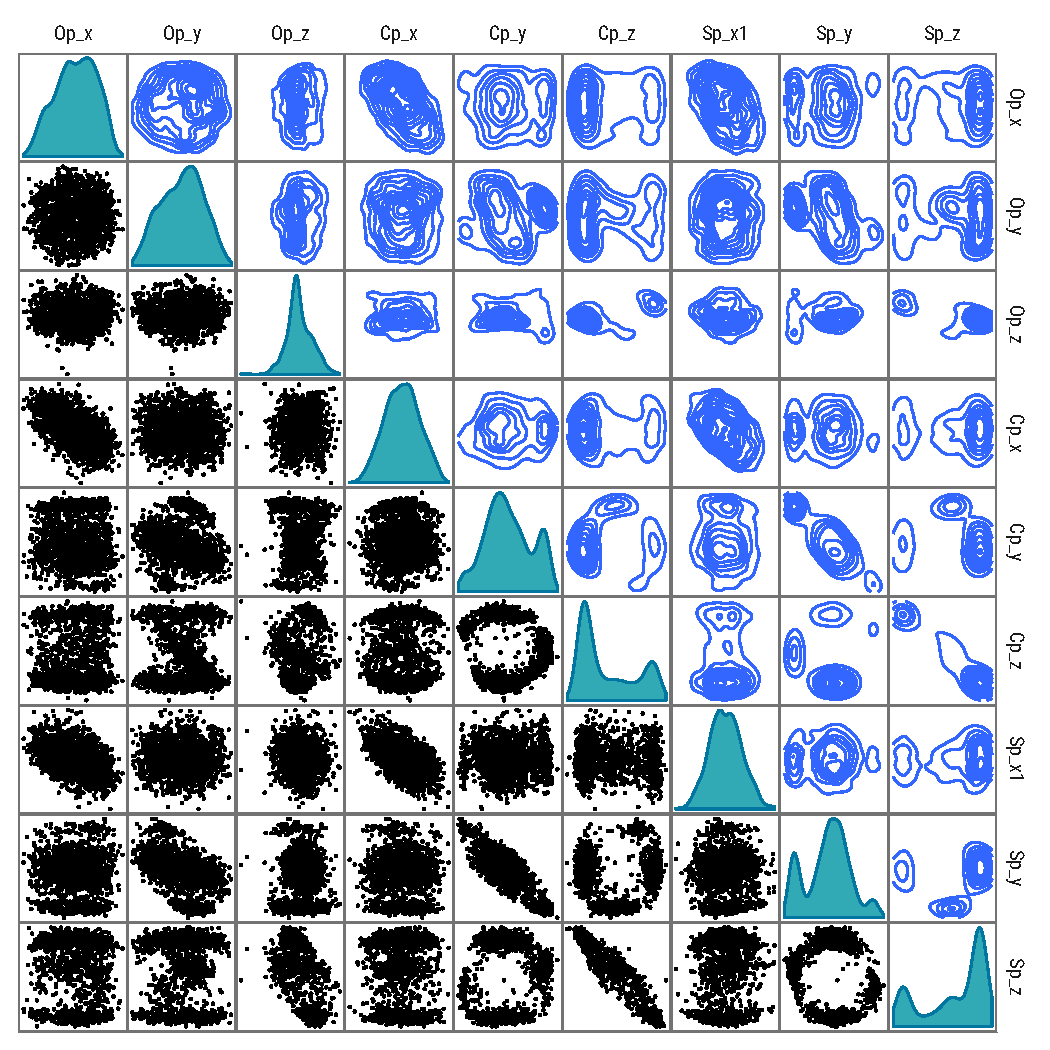
\includegraphics[width=\textwidth]{Plots/OCS2227fsMomentumPairPlots}
  \caption[OCS (2,2,2) 7fs momentum pair plots.]
  {OCS (2,2,2) 7fs momentum pair plots.}
  \label{fig:OCS2227fsMomentumPairPlots}
\end{figure}
\clearpage

% Implementation (+ extra convergence cube)
\section{Implementation}
\index{Lookup table}
\index{Geometry reconstruction!Lookup table}
In this approach, many Coulomb explosions are simulated (see secton \ref{sec:simulating}) using a wide variety of molecular structures as the initial condition, and the resulting momentum vectors from each simulation are stored. Thus you have a mapping from molecular structures to momentum vectors. To determine the structure belonging to a certain set of observed momentum vectors, you simply read the table in reverse. This approach is simple to implement, very quick by design, and front-loads the computation which may be desirable for large data sets. However, of course, it has an exponential time and space complexity $\mathcal{O}(e^{3N-6})$ where $N$ is the number of atoms.

\subsection{Using simulations to test accuracy}
It is important that we do not simulate geometries that are already contained in the lookup table.

\subsection{Computational complexity}

\section{Geometry reconstructions done by lookup table}

\pagebreak
\begin{figure}
  \centering
  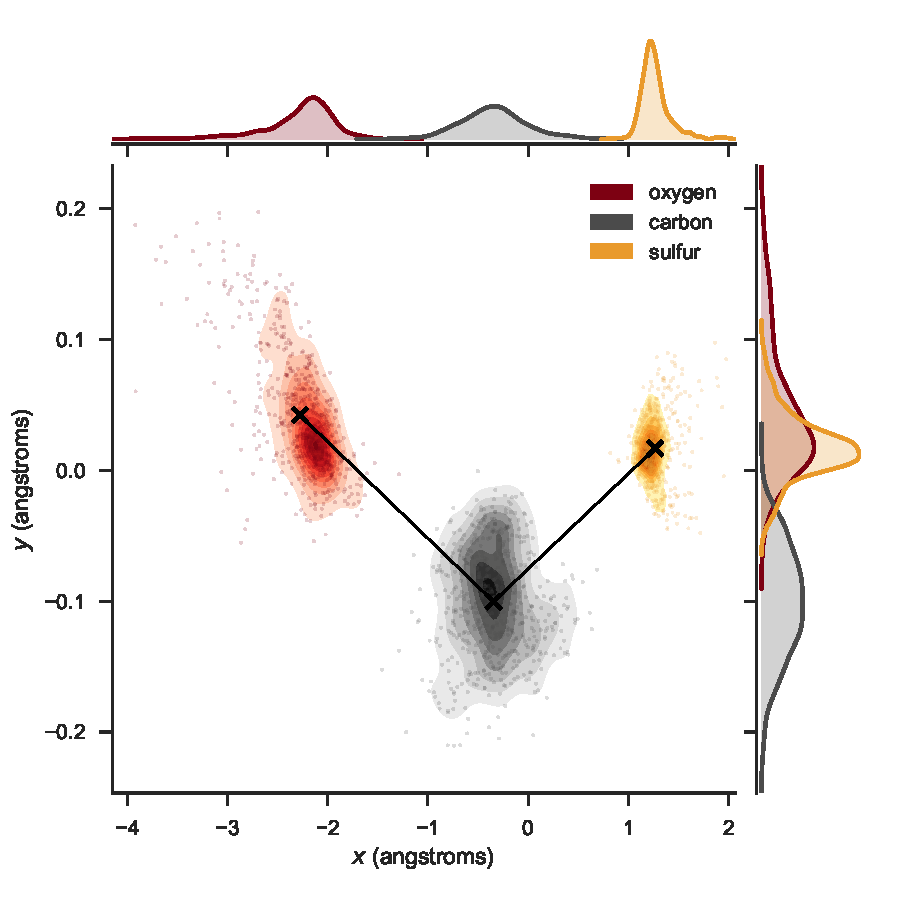
\includegraphics[width=\textwidth]{Plots/OCS2227fsLTGeometry}
  \caption[OCS (2,2,2) 7fs lookup table geometry.]
  {OCS (2,2,2) 7fs lookup table geometry.}
  \label{fig:OCS2227fsLTGeometry}
\end{figure}

It probably does not matter how geometries are plotted. 

\clearpage

\section{Conclusions and lessons learnt}
\subsection{Precision is computationally expensive}
\subsection{Difficulty in scaling to larger molecules}

\pagebreak
\subsection{Degenerate molecular structures}
We have previously hinted at the fact that due to the ill-posed nature of the geometry reconstruction inverse problem, multiple solutions may be posible. This feature actually does pop up for the OCS molecule and the lookup table is perhaps the best method of investigating these multiple solutions, which we will call degenerate geometries.

\begin{figure}
  \centering
  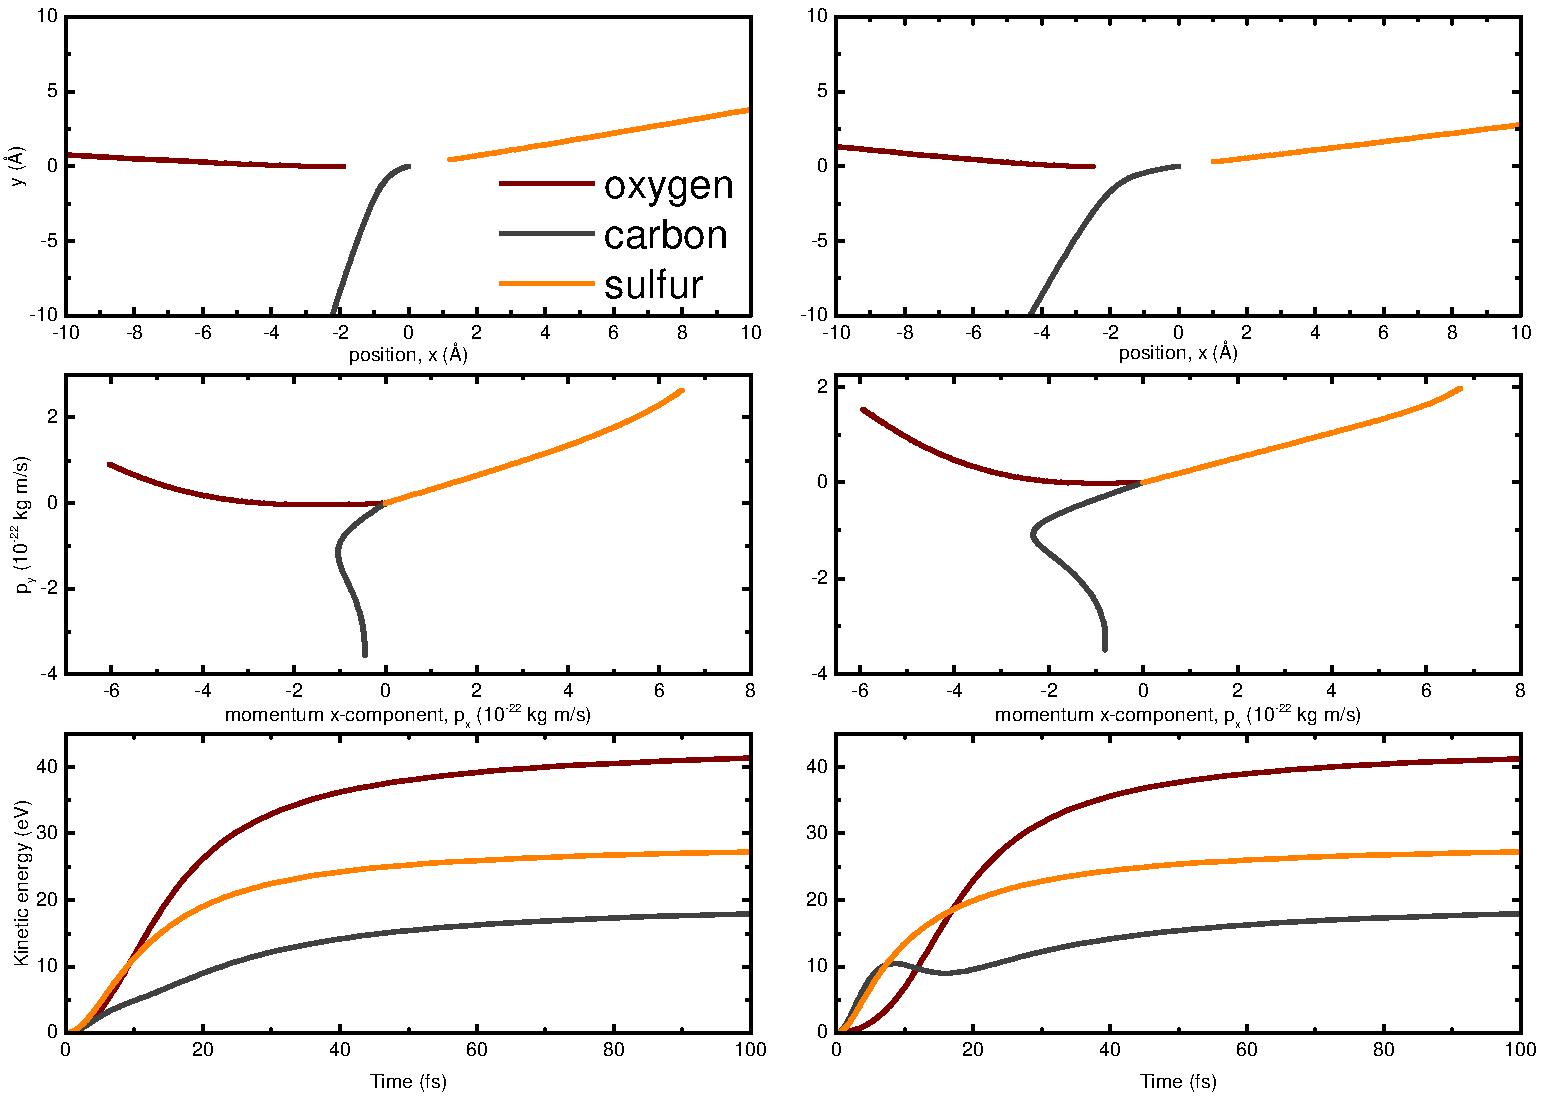
\includegraphics[width=\textwidth]{Plots/DegenerateGeometryTrajectories.pdf}
  \caption[Degenerate geometry trajectories.]
  {Degenerate geometry trajectories.}
  \label{fig:DegenerateGeometryTrajectories}
\end{figure}
\clearpage

\section{Future usefulness}

% Another warning box that zooming in doesn't actually help much. If you're
% near a local minimum, you'll just zoom into that. A first go usually gives you ~ 2 sig figs of precision, anything more doesn't mean much as our momentum uncertainty is pretty high.
% Warning awesomebox that the MATLAB code has not been vectorized.